\chapter[Manual de usuario]{
  \label{chp:manualdeusuario}
  MANUAL DE USUARIO
}
\thispagestyle{numberingStyle}
\pagestyle{numberingStyle}


\section{Manual de usuario aplicación móvil}

\subsection*{Acceso a la aplicación}
\begin{figure}[H]
\centering
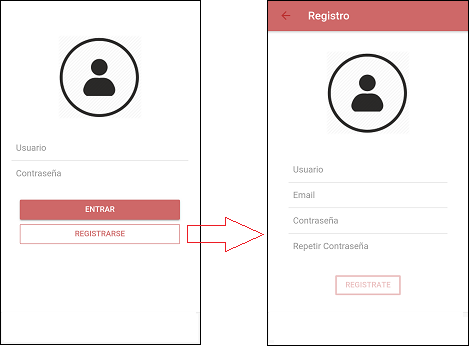
\includegraphics[
   keepaspectratio=true
]{./11_Apendice/Apendice_B/img/Ionic-1-Login.png}
\caption{Pantalla acceso - Aplicación móvil.}
\end{figure}

Cuando se accede a la aplicación por primera vez se mostrará la pantalla que aparece en la parte izquierda de la figura anterior. El usuario, si ya tiene una cuenta registrada, deberá ingresar los datos de acceso y darle al botón de \textit{Entrar} para acceder a la aplicación. Si el usuario no se encuentra registrado deberá darse de alta en la aplicación haciendo click sobre el botón \textit{Registrarse}. Al registrarse, se mostrará el formulario que aparece a la derecha de la imagen, solicitando los datos necesarios. El sistema validará los datos de entrada y procederá a la autenticación del usuario.


\subsection*{Pantalla principal}

La pantalla principal de la aplicación estará formada por tres pestañas, que son las siguientes:


\begin{figure}[H]
\centering
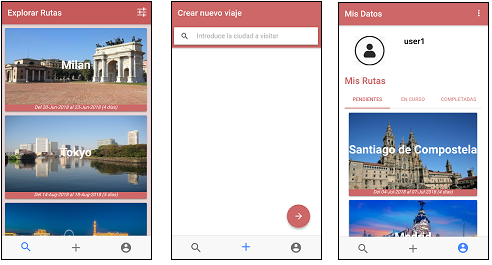
\includegraphics[
   keepaspectratio=true
]{./11_Apendice/Apendice_B/img/Ionic-2-Tabs.png}
\caption{Pantalla principal - Aplicación móvil.}
\end{figure}

De izquierda a derecha, y mediante el selector que aparece en la parte inferior, se puede alternar entre las pestañas de \textit{Explorar Rutas}, \textit{Crear Ruta} y \textit{Mis Datos}.


\newpage
\subsubsection*{Explorar Rutas}

La pestaña de explorar rutas permitirá consultar las rutas creadas por los demás usuarios.

\begin{figure}[H]
\centering
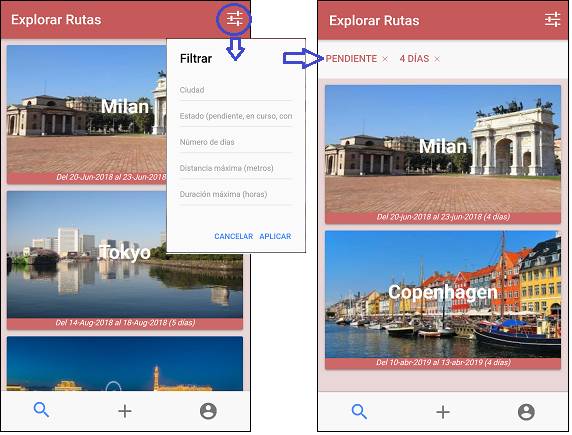
\includegraphics[
   keepaspectratio=true
]{./11_Apendice/Apendice_B/img/Ionic-3-ExploreRoutes.png}
\caption{Pantalla explorar - Aplicación móvil.}
\end{figure}

En el cuerpo de la pestaña aparece el listado con las rutas de los usuarios. Para cada una de ellas, se muestra una imagen de fondo de la ciudad de destino, su nombre y las fechas establecidas. En la parte superior derecha de la pestaña existe la opción de aplicar un filtro sobre las rutas. Al hacer click sobre dicho botón se mostrará el formulario en el que se podrá indicar ciudad, estado, número de días, distancia máxima o duración máxima para filtrar.

Los filtros son acumulativos y se pueden ver los activos en la parte superior de la pantalla.


\subsubsection*{Crear nuevo viaje}
\begin{figure}[H]
\centering
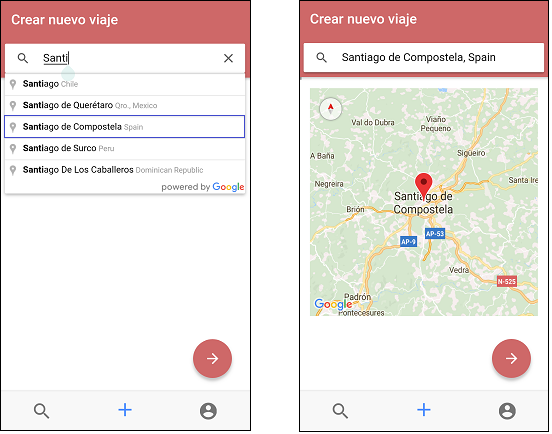
\includegraphics[
   keepaspectratio=true
]{./11_Apendice/Apendice_B/img/Ionic-4-AddRoute.png}
\caption{Pantalla crear - Aplicación móvil.}
\end{figure}


La pantalla para crear rutas ofrecerá, en la parte superior, un buscador de ciudades. Al buscar una ciudad, el sistema ayudará autocompletando con las ciudades disponibles, obtenidas de Google. Al seleccionar una de ellas, se mostrará un mapa, indicando la ubicación geográfica de dicha ciudad.

Haciendo click en la flecha de la parte inferior de la pantalla, se da de alta la ruta en el sistema, y si no se produce ningún error, se redirige al usuario a la vista encargada de mostrar la información detallada de la ruta.

\newpage
\subsubsection*{Mis Datos}
En esta pestaña, se muestran los datos del usuario conectado a la aplicación. En la parte superior de la pantalla aparece un botón de opciones que permite modificar los datos del usuario y desconectarse de la aplicación. Ambas acciones, mostrarán respectivamente los formularios, situados a la derecha en la siguiente figura.

\begin{figure}[H]
\centering
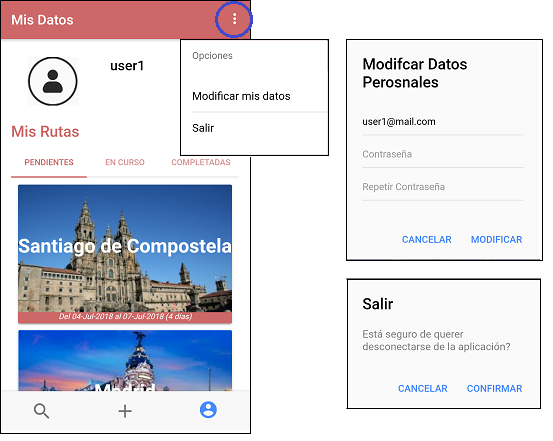
\includegraphics[
   keepaspectratio=true
]{./11_Apendice/Apendice_B/img/Ionic-5-MyData.png}
\caption{Pantalla mis datos - Aplicación móvil.}
\end{figure}


Para modificar los datos de usuario será necesario indicar correo electrónico y contraseña a modificar. Si el usuario confirma los datos, el sistema realizará las validaciones y actualizará los datos del usuario en el sistema.

En la parte central de la pantalla aparece la información sobre las rutas creadas por dicho usuario. En el listado, se puede hacer uso del selector que permite clasificar dichas rutas en función de su estado (pendientes, en curso o completadas). Con un click sobre las rutas, se podrá acceder y consultar detalladamente la ruta seleccionada.


\newpage
\subsection*{Panel de viaje}
Una vez creada una ruta o cuando se consulta, se mostrará el siguiente panel que permitirá personalizarla.


\begin{figure}[H]
\centering
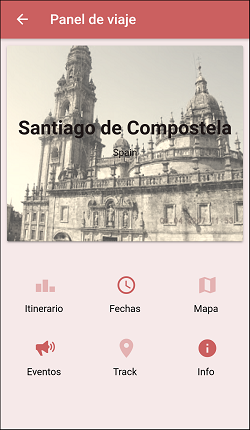
\includegraphics[
   keepaspectratio=true
]{./11_Apendice/Apendice_B/img/Ionic-6-RoutePanel.png}
\caption{Pantalla panel de viaje - Aplicación móvil.}
\end{figure}

Este panel se compone de:

\begin{itemize}
	\item \textbf{Itinerario. }Opción que permite consultar la distribución por días de la ruta.
	
	\item \textbf{Fechas. }Acción para asignar una rango de fechas a la ruta.
	
	\item \textbf{Mapa. }Muestra el itinerario de la ruta haciendo uso de mapas.
	
	\item \textbf{Eventos. }Permite consultar los eventos disponibles en la ciudad donde se va realizar el viaje. 
	
	\item \textbf{Track. }Activa la geolocalización, que permitirá guardar la información en tiempo real de la ruta.
	
	\item \textbf{Info. }Muestra los detalles de la ruta.
\end{itemize}

Los elementos ensombrecidos estarán deshabilitados mientras no se asignen las fechas al viaje.


\subsubsection*{Fechas}

Lo primero a realizar es asignar unas fechas al viaje.

\begin{figure}[H]
\centering
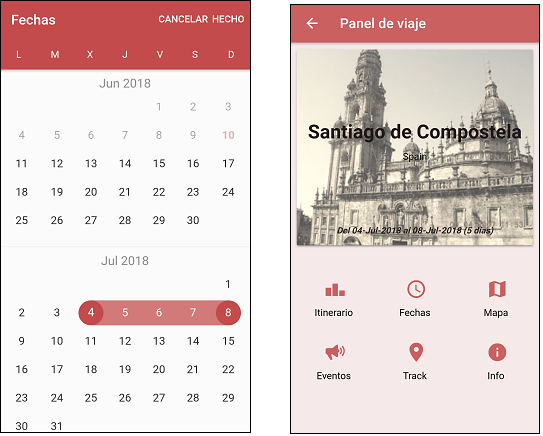
\includegraphics[
   keepaspectratio=true
]{./11_Apendice/Apendice_B/img/Ionic-7-Dates.png}
\caption{Pantalla fechas - Aplicación móvil.}
\end{figure}

Al hacer click sobre la opción \textit{Fechas} del panel, se abrirá una ventana en la que se podrá seleccionar el rango de fechas en las que se va realizar el viaje. Una vez asignadas las fechas, en el panel, la opción \textit{Itinerario} ya estará disponible.


\subsection*{Itinerario}
La página del itinerario será la encargada de mostrar las visitas asignadas a los días de la ruta. En el siguiente ejemplo se mostrarán dos días de la ruta con unas visitas ya agregadas.

\begin{figure}[H]
\centering
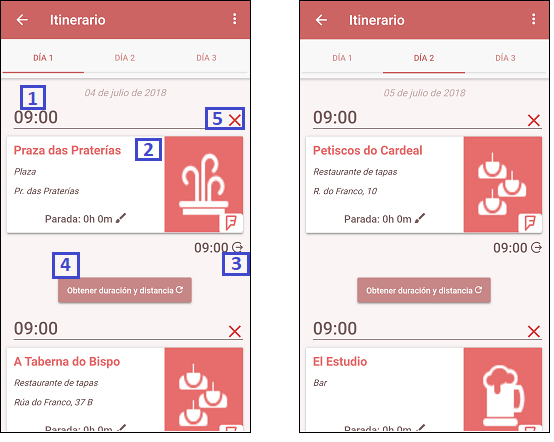
\includegraphics[
   keepaspectratio=true
]{./11_Apendice/Apendice_B/img/Ionic-8-Itinerario.png}
\caption{Pantalla itinerario - Aplicación móvil.}
\end{figure}

El selector de la parte superior permite obtener las visitas asignadas a los diferentes días de la ruta. En el cuerpo de la página, aparece el listado con las visitas y la información  relevante en cada una de ellas.

\begin{itemize}
	\item \textbf{1. }Hora de llegada al lugar, en la primera visita corresponde con la hora de comienzo del día de la ruta, valor modificable por el usuario. 	
	
	\item \textbf{2. }Datos relevantes del lugar en concreto. Al final del bloque, incluye un apartado denominado \textit{Parada}, donde se especificará el tiempo que se pasará en dicho lugar. 
	
	\item \textbf{3. }Indica la hora de salida del sitio, calculada en función del tiempo que desea pasar el usuario en el sitio.
	
	\item \textbf{4. }Acción que permite obtener la distancia y duración que hay entre dos visitas.
	
	\item \textbf{5. }Acción para eliminar una visita concreta del itinerario.
\end{itemize}

\subsubsection*{Calcular duración y distancia}

Al hacer click en el botón para obtener la distancia entre dos visitas obtenemos el siguiente resultado.

\begin{figure}[H]
\centering
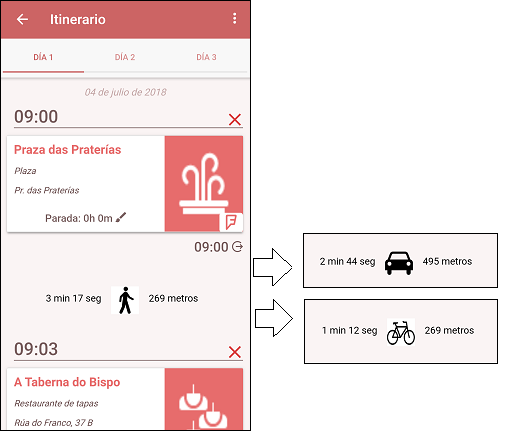
\includegraphics[
   keepaspectratio=true
]{./11_Apendice/Apendice_B/img/Ionic-9.png}
\caption{Pantalla calcular distancia - Aplicación móvil.}
\end{figure}

Como se puede observar en la imagen, ahora aparecen calculados los tiempos de desplazamiento y la duración entre las dos visitas. Haciendo ahora click sobre esa información obtenida, el sistema alterna los métodos de transporte disponibles, junto con la información obtenida para cada uno. En la figura se muestran los tres métodos de transporte que se utilizan, junto con la información de cada uno de ellos.


\subsubsection*{Modificar tiempo parada}
El tiempo a parar en cada visita se puede modificar haciendo click sobre el icono en forma de lápiz que aparece dentro de la información de cada visita.

\begin{figure}[H]
\centering
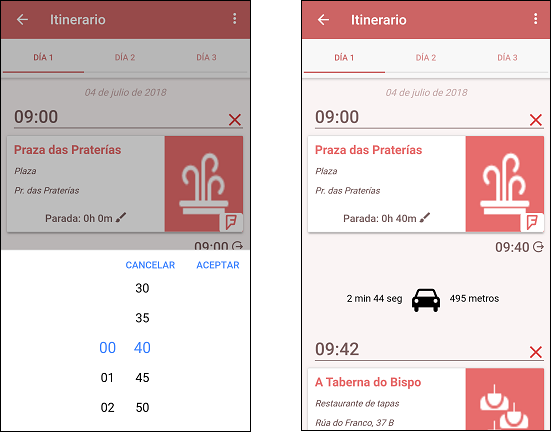
\includegraphics[
   keepaspectratio=true
]{./11_Apendice/Apendice_B/img/Ionic-10.png}
\caption{Pantalla modificar tiempo parada - Aplicación móvil.}
\end{figure}

En la ventana emergente se podrá seleccionar el tiempo a pasar en la visita seleccionada, indicando las horas  en la columna de la izquierda y los minutos en la de la derecha. 

Una vez actualizada dicha información, se mostrará el tiempo indicado en la información de la visita y se recalcularán los tiempos de salida y llegada en las visitas posteriores.


\subsubsection*{Opciones itinerario}
En la parte superior aparece un icono con tres puntos verticales que nos permitirán acceder a las opciones del día concreto de la ruta.

\begin{figure}[H]
\centering
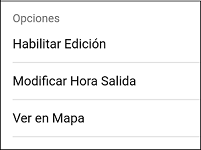
\includegraphics[
   keepaspectratio=true
]{./11_Apendice/Apendice_B/img/Ionic-11.png}
\caption{Pantalla opciones itinerario - Aplicación móvil.}
\end{figure}


\begin{itemize}
	\item \textbf{Habilitar Edición. }Permitirá editar el orden de las visitas en el día concreto.
	
	\begin{figure}[H]
\centering
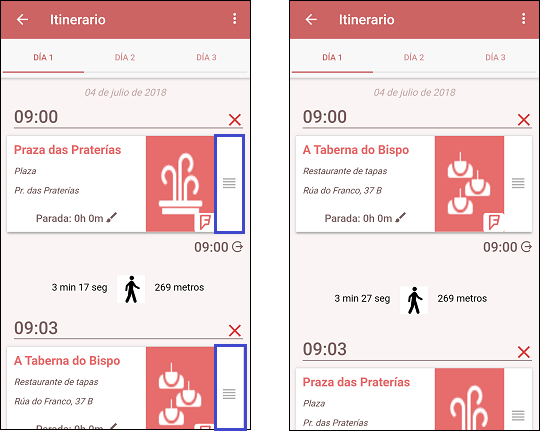
\includegraphics[
   keepaspectratio=true
]{./11_Apendice/Apendice_B/img/Ionic-12.png}
\caption{Pantalla editar itinerario - Aplicación móvil.}
\end{figure}

	Al seleccionar la opción de edición, aparecerá al lado de cada visita un selector que permitirá coger y arrastrar cada visita a la posición deseada.	
	
	\item \textbf{Modificar Hora Salida. } Esta opción permitirá modificar la hora de comienzo de la primera visita del día.
	
		\begin{figure}[H]
\centering
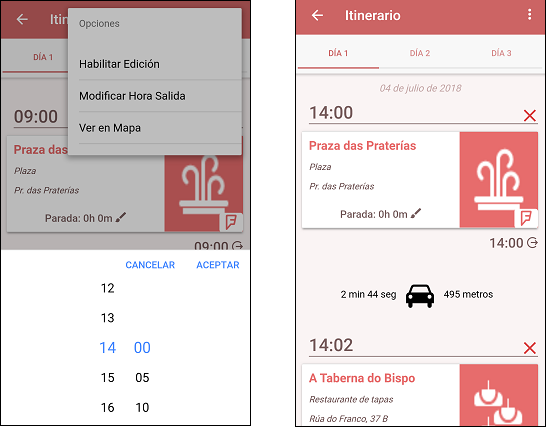
\includegraphics[
   keepaspectratio=true
]{./11_Apendice/Apendice_B/img/Ionic-13.png}
\caption{Pantalla modificar hora salida - Aplicación móvil.}
\end{figure}

	Al igual que ocurría con los tiempos de parada en las visitas, la asignación de la hora de comienzo sigue el mismo sistema de selección.
	
	\item \textbf{Ver en Mapa. }Permitirá consultar el día de la ruta en el mapa.
	
	
	
\begin{figure}[H]
\centering
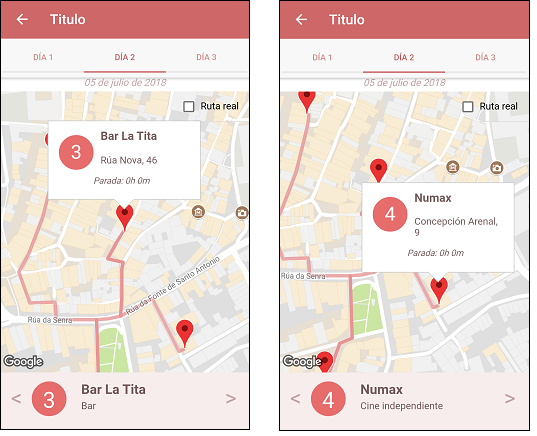
\includegraphics[
   keepaspectratio=true
]{./11_Apendice/Apendice_B/img/Ionic-14.png}
\caption{Pantalla mapa - Aplicación móvil.}
\end{figure}
\end{itemize}

El mapa podrá ser consultado directamente tanto desde el itinerario como desde el panel principal de la ruta. Si se hace desde la pantalla \textit{Itinerario}, se mostrará el día seleccionado como primera opción. Si se consulta desde el panel de la ruta, se mostrará de inicio el mapa del primer día de la ruta. Dentro de la pantalla, se podrá alternar los días mediante el selector superior, al igual que se hacía en la pantalla de \textit{Itinerario}.
	
	En el mapa aparecerán marcadas las visitas a realizar en el día concreto. Si se hace click sobre dichas marcas, se abrirá una ventana con información más detallada de la visita, indicando su orden, nombre, dirección y tiempo de parada.
	
	En la parte inferior, se encuentra una lista con todos las visitas para el día determinado. Mediante desplazamiento horizontal, se podrán alternar entre las diferentes visitas y, al cambiar a otra, automáticamente se mostrará su ventana de información en el mapa.
	
	
En la parte superior derecha de la imagen anterior, aparece un botón seleccionable que permite incorporar al mapa los datos reales de la ruta, si es que los hubiese. Al hacer click sobre ese botón, se incluiría en el mapa una nueva ruta formada por las ubicaciones que ha recorrido el usuario en determinado día.

\begin{figure}[H]
\centering
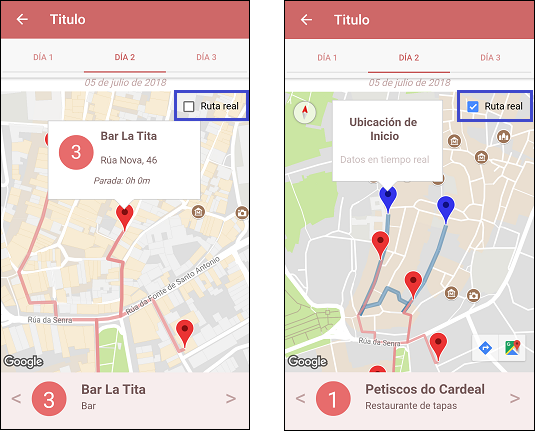
\includegraphics[
   keepaspectratio=true
]{./11_Apendice/Apendice_B/img/Ionic-20.png}
\caption{Pantalla mapa tiempo real - Aplicación móvil.}
\end{figure}

En la figura se puede observar en color rojo la ruta planificada con los sitios establecidos y, en color azul, la ruta real hecha por el usuario, compuesta de punto de inicio y fin.


\newpage
\subsection*{Eventos}
En la pantalla \textit{Panel de viaje} se podrán consultar los eventos disponibles.

\begin{figure}[H]
\centering
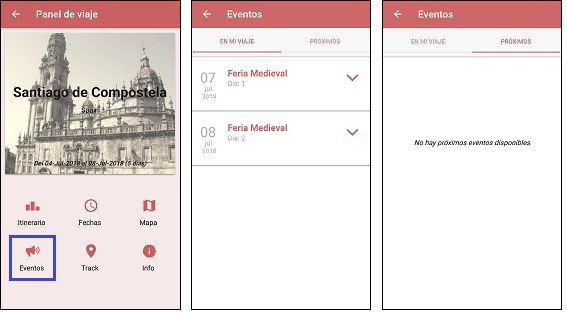
\includegraphics[
   keepaspectratio=true
]{./11_Apendice/Apendice_B/img/Ionic-15.png}
\caption{Pantalla eventos - Aplicación móvil.}
\end{figure}

Haciendo click sobre \textit{Eventos}, abriremos la pantalla de eventos donde, mediante el selector, podremos obtener los eventos coincidentes en nuestro viaje así como los eventos futuros que se celebren en la misma ciudad. 

\begin{figure}[H]
\centering
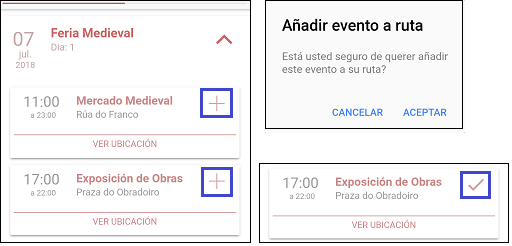
\includegraphics[
   keepaspectratio=true
]{./11_Apendice/Apendice_B/img/Ionic-16.png}
\caption{Pantalla añadir evento - Aplicación móvil.}
\end{figure}


Al desplegar un evento en concreto de los mostrados, se muestran las diferentes actividades o localizaciones que componen dicho evento. Seleccionando el botón con el signo `+' indicado en la figura, se añadirá dicha actividad al día correspondiente de la ruta. Una vez añadida la actividad, aparecerá con un símbolo como una `V', indicando que esa actividad ya está asignada. Volviendo hacer click sobre ella podremos eliminarla de la ruta.

La opción \textit{Ver Ubicación} permitirá mostrar la ubicación de la actividad en el mapa y compararla con la ruta elaborada. 

\begin{figure}[H]
\centering
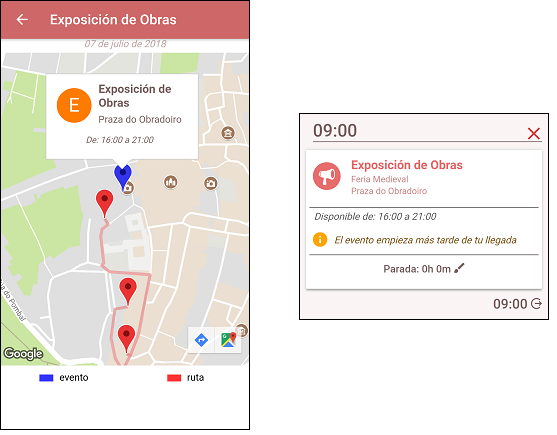
\includegraphics[
   keepaspectratio=true
]{./11_Apendice/Apendice_B/img/Ionic-17.png}
\caption{Pantalla mapa evento - Aplicación móvil.}
\end{figure}

La imagen de la izquierda de la figura anterior muestra la pantalla donde se puede consultar el evento en el mapa mientras que la de la derecha muestra como se representaría un evento en el itinerario de un día de la ruta. 


\newpage
\subsection*{Activar geolocalización}
En el panel de viaje, podremos activar la geolocalización cuando la ruta se encuentre en algunos de los días para los cuáles está planificada. Haciendo click sobre el botón que pone \textit{Track}, el sistema activará automáticamente la geolocalización en segundo plano. Se sabrá que está activa por el cambio de color en el icono y, simplemente haciendo click de nuevo sobre el icono, podrá desactivarse.


\begin{figure}[H]
\centering
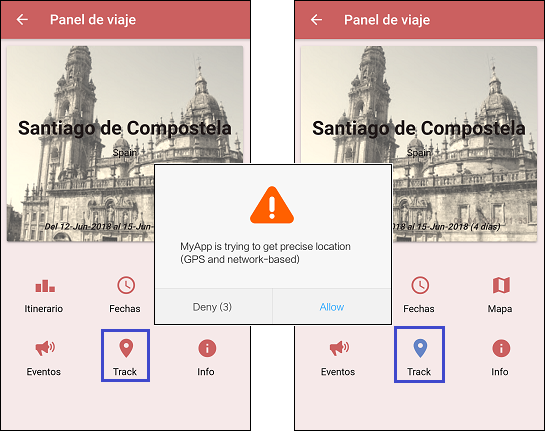
\includegraphics[
   keepaspectratio=true
]{./11_Apendice/Apendice_B/img/Ionic-18.png}
\caption{Pantalla activar geolocalización - Aplicación móvil.}
\end{figure}

Será necesario otorgar permisos de acceso al GPS para su correcto funcionamiento.

\newpage
\subsection*{Pantalla información}
Desde el panel principal se podrá acceder a la información relevante de la ruta a través de la opción \textit{Info}.


\begin{figure}[H]
\centering
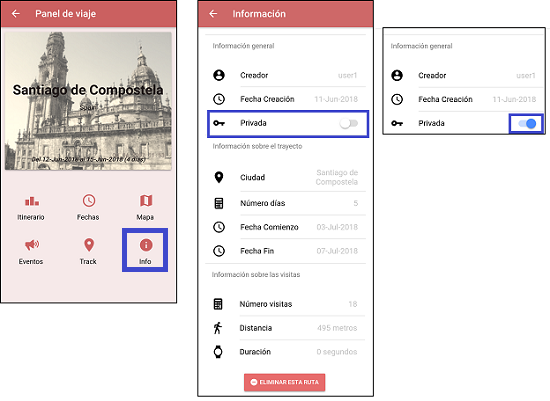
\includegraphics[
   keepaspectratio=true
]{./11_Apendice/Apendice_B/img/Ionic-19.png}
\caption{Pantalla información viaje - Aplicación móvil.}
\end{figure}

En esta pantalla se muestra toda la información relacionada con la ruta y, haciendo uso de la opción \textit{Privada}, se puede alternar la privacidad establecida para la ruta.


\newpage
\subsection*{Añadir lugares}
Para añadir lugares a visitar en una ruta, será necesario hacerlo desde la pantalla de \textit{Itinerario}. Al final de la lista de visitas tendremos la opción de incorporar un nuevo lugar.

\begin{figure}[H]
\centering
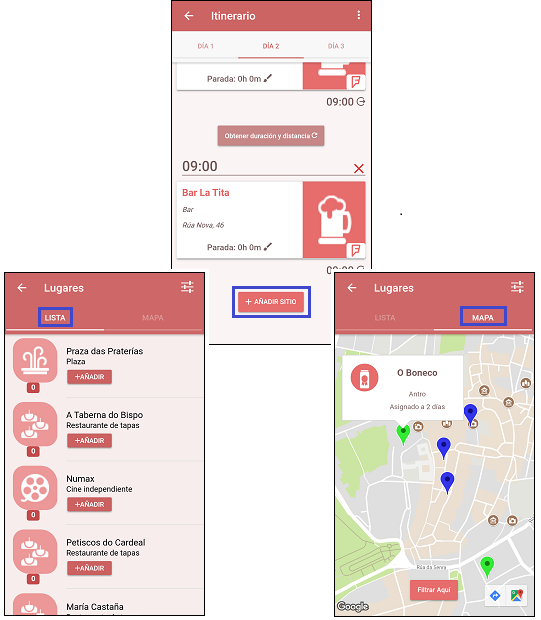
\includegraphics[
   keepaspectratio=true
]{./11_Apendice/Apendice_B/img/Ionic-21.png}
\caption{Pantalla lugares - Aplicación móvil.}
\end{figure}

Al hacer click en \textit{Añadir Sitio}, automáticamente se muestran los sitios recomendados en esa ciudad. A la hora de visualizarlos, tenemos dos opciones, mediante lista o en un mapa. En la lista, aparecerá un número debajo de cada sitio que indicará el número de días a los que ya está asignado ese lugar. En el mapa, esta información se podrá saber haciendo click en la marca generada para cada sitio. Las marcas verdes del mapa indicarán que el sitio ya está incorporado a algún día del viaje mientras que las azules indicarán lo contrario. 

Mediante el botón \textit{Filtrar Aquí}, situado en la parte inferior del mapa, se podrán aplicar los filtros de búsqueda en una zona del mapa determinada. 

Haciendo click en la opción \textit{Añadir}, existente en cada uno de los elementos de la lista de lugares, se podrán añadir dichos lugares a la ruta. 

\begin{figure}[H]
\centering
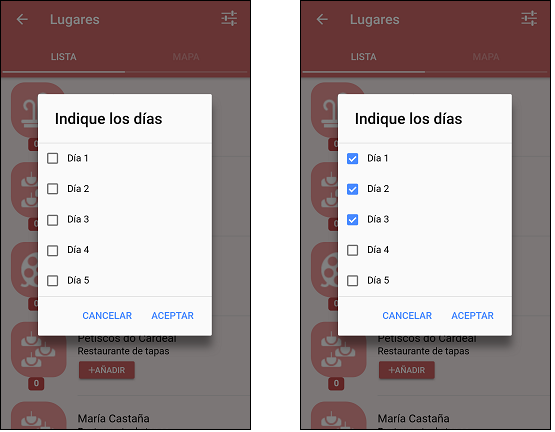
\includegraphics[
   keepaspectratio=true
]{./11_Apendice/Apendice_B/img/Ionic-23.png}
\caption{Pantalla añadir lugar - Aplicación móvil.}
\end{figure}

Se mostrará una ventana con el número de días que forman la ruta de viaje. Seleccionando y deseleccionando los días, se añadirá o eliminará, respectivamente, el lugar en dichos días.


Por su parte, los filtros se podrán consultar y/o modificar en el botón situado en la parte superior derecha. Con un click sobre el, se mostrará el siguiente menú.

\begin{figure}[H]
\centering
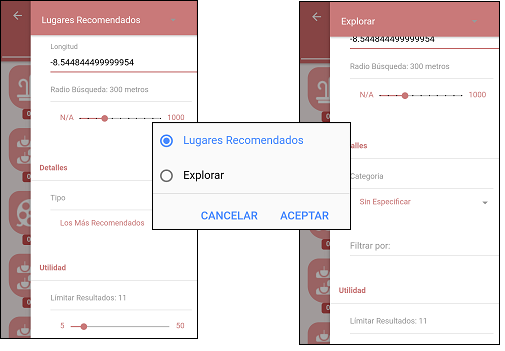
\includegraphics[
   keepaspectratio=true
]{./11_Apendice/Apendice_B/img/Ionic-22.png}
\caption{Pantalla filtrar lugares - Aplicación móvil.}
\end{figure}


En dicho menú, en su parte superior, se puede seleccionar entre las opciones: \textit{Lugares Recomendados} y \textit{Explorar}, que ofrecerán una serie de filtros diferentes. En concreto, en la opción \textit{Explorar} se podrá hacer uso de las categorías obtenidas de la fuente externa. En la parte inferior del menú, se situará un botón que servirá para aplicar dichos filtros.


\newpage
\section{Manual de usuario aplicación web}

\subsection{Acceso a la aplicación}

Tanto la aplicación web de usuario como la aplicación web de administración tendrán el mismo punto de acceso, que será el siguiente:

\begin{figure}[H]
\centering
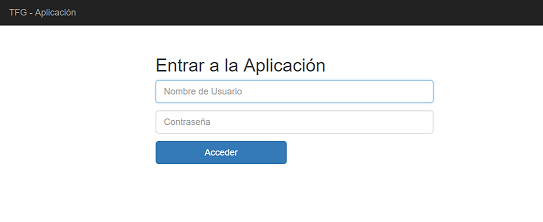
\includegraphics[
   keepaspectratio=true
]{./11_Apendice/Apendice_B/img/WebLogin.png}
\caption{Pantalla acceso - Aplicación web.}
\end{figure}

Se mostrará un pequeño formulario en el que será necesario indicar usuario y contraseña para poder acceder a la aplicación. En función del rol del usuario, se accederá al panel de administración o a la propia aplicación de usuario. 

\subsection{Aplicación de usuario}

\subsubsection*{Pantalla principal}
Si se accede a la aplicación de usuario se mostrará la siguiente pantalla:

\begin{figure}[H]
\centering
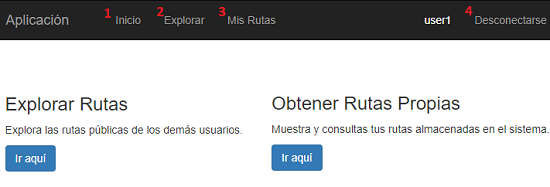
\includegraphics[
   keepaspectratio=true
]{./11_Apendice/Apendice_B/img/WebIndex.png}
\caption{Pantalla principal - Aplicación usuario}
\end{figure}

La barra de navegación será fija para todas las pantallas de la aplicación de usuario y estará formada por:

\begin{itemize}
	\item \textbf{1 - \textit{Inicio}}. Dirige al usuario a esta página.
	\item \textbf{2 - \textit{Explorar}}. Dirige al usuario a la pantalla donde podrá explorar las rutas, de los demás usuarios existentes en la aplicación.
	\item \textbf{3 - \textit{Mis Rutas}}. Dirige al usuario a la pantalla donde podrá consultar las rutas creadas por él mismo.
	\item \textbf{4 - \textit{Desconectarse}}. Permite al usuario desloguearse de la aplicación. Al lado, aparece el nombre de usuario que está actualmente conectado.
\end{itemize}
	
	
En el cuerpo de la página aparecen detalladas las funcionalidades que puede realizar el usuario. En este caso, esas funcionalidades son las mismas que se encuentran en los puntos 2 y 3 de la barra de navegación, \textit{Explorar} y \textit{Mis Rutas}, respectivamente.


\subsubsection*{Explorar rutas}
\begin{figure}[H]
\centering
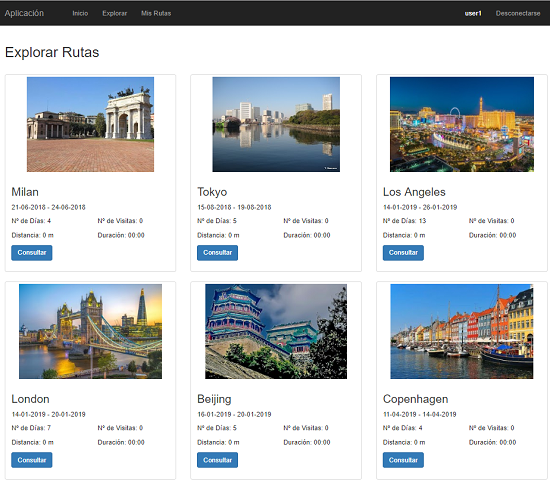
\includegraphics[
   keepaspectratio=true
]{./11_Apendice/Apendice_B/img/WebExploreRoutes.png}
\caption{Pantalla explorar rutas - Aplicación usuario}
\end{figure}

La pantalla de explorar rutas permitirá al usuario obtener las rutas públicas creadas por los demás usuarios de la aplicación. Indicará un listado de las rutas con una pequeña información sobre cada una ellas y cada elemento de la lista incluirá la opción de consultar, que permitirá acceder a la vista de detalles. 

Esta pantalla sigue, visualmente, un estilo similar a la pantalla de \textit{Mis Rutas}, que veremos a continuación más detalladamente. 


\subsubsection*{Mis rutas}

Dentro de la página \textit{Mis Rutas}, el usuario podrá obtener las rutas creadas por él, clasificadas en función de su estado.

\begin{figure}[H]
\centering
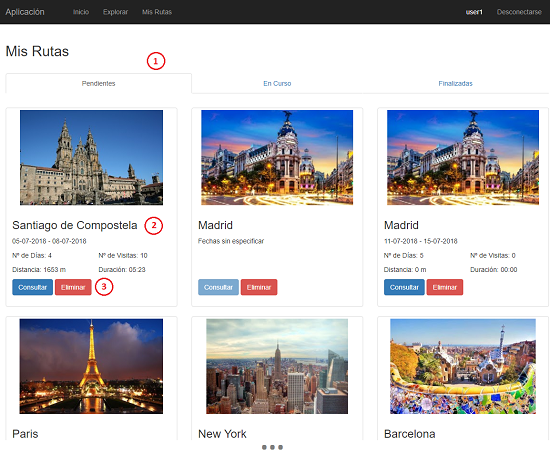
\includegraphics[
   keepaspectratio=true
]{./11_Apendice/Apendice_B/img/WebMyRoutes.png}
\caption{Pantalla mis rutas - Aplicación usuario}
\end{figure}

\begin{itemize}
	\item \textbf{Zona 1.} Selector que permite alternar entre las rutas, clasificadas por los diferentes estados en los que se encuentran.
	\item \textbf{Zona 2.} Bloque que representa la información básica de la ruta. Incluye foto, nombre de la ciudad, fechas, número de días, número de visitas asignadas y distancia y duración totales.
	\item \textbf{Zona 3.} Acciones a realizar sobre determinada ruta.
	\begin{itemize}
		\item Si el usuario selecciona \textit{Eliminar}, se mostrará una alerta, indicando al usuario si desea confirmar o no la acción solicitada.
		\begin{figure}[H]
			\centering
			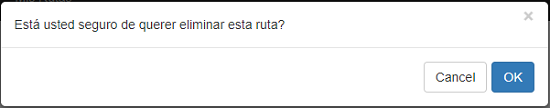
\includegraphics[
			   keepaspectratio=true
			]{./11_Apendice/Apendice_B/img/WebMyRoutesDelete.png}
			\caption{Pantalla eliminar ruta - Aplicación usuario}
		\end{figure}


			
		\item Si el usuario selecciona \textit{Consultar}, el sistema lo dirigirá a la pantalla de \textit{Detalles}, donde podrá obtener la información, detallada por días, de la ruta seleccionada.
	\end{itemize}			
\end{itemize}


\subsubsection*{Detalles ruta}
\begin{figure}[H]
\centering
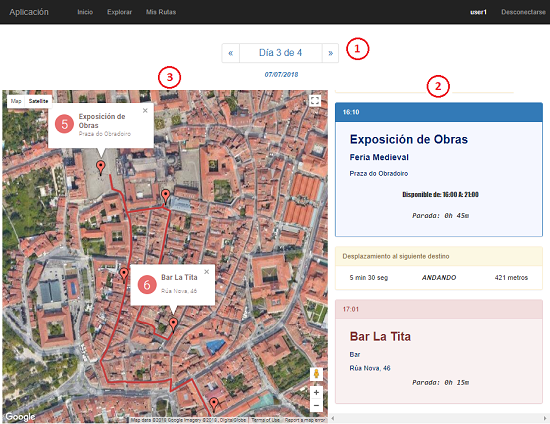
\includegraphics[
	keepaspectratio=true
]{./11_Apendice/Apendice_B/img/WebDetailRoute.png}
\caption{Pantalla detalles ruta - Aplicación usuario}
\end{figure}

En la página de detalles de la ruta tenemos tres zonas diferenciadas:

\begin{itemize}
	\item \textbf{Zona 1. }Selector que permite navegar por los días de la ruta.
	\item \textbf{Zona 2. }Listado, por orden, con los lugares a visitar en determinado día. Cada visita incluye el tiempo de llegada y una pequeña descripción con el nombre del lugar o evento, dirección y tiempo de parada. Se hace distinción por colores, en azul se muestran las visitas a eventos, en rojo las visitas a lugares y en amarillo se indica la información de distancia y tiempo entre cada uno de ellos.
	\item \textbf{Zona 3. }Mapa en el que se muestran las visitas del listado anterior. Haciendo click en cada marca, se abre una ventana de información, en la que se indica el orden que ocupa dicha visita en la ruta, su nombre y la dirección. Al tratarse de un mapa de Google, se puede interactuar con las funcionalidades que este ofrece, como son la vista en satélite o en mapa, hacer uso del StreetView, etc.
\end{itemize}


\subsection{Panel de administración}

\subsubsection*{Barra de navegación}

\begin{figure}[H]
\centering
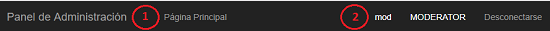
\includegraphics[
   keepaspectratio=true
]{./11_Apendice/Apendice_B/img/WebPanelNavBar.png}
\caption{Barra de navegación - Panel de administración}
\end{figure}

La barra de navegación está formada por:

\begin{itemize}
	\item \textbf{1 - Página principal}. Dirige al usuario a la página principal.
	\item \textbf{2 - Información de usuario}. Se mostrará el nombre del usuario conectado junto al rol que desempeña. A la derecha de todo se incluye la opción para desconectarse de la aplicación.
\end{itemize}


\subsubsection*{Pantalla principal}
Si el usuario que accede a la aplicación, tiene rol de administrador o de gestor de eventos, se mostrarán respectivamente las siguientes pantallas.

\begin{figure}[H]
\centering
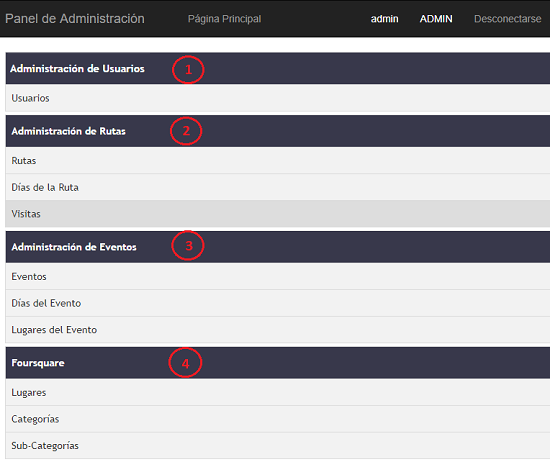
\includegraphics[
   keepaspectratio=true
]{./11_Apendice/Apendice_B/img/WebPanelIndexAdmin.png}
\caption{Pantalla principal administrador - Panel de administración}
\end{figure}


\begin{figure}[H]
\centering
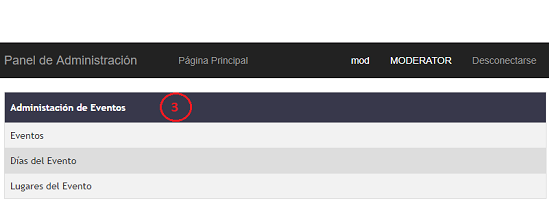
\includegraphics[
   keepaspectratio=true
]{./11_Apendice/Apendice_B/img/WebPanelIndexMod.png}
\caption{Pantalla principal gestor de eventos - Panel de administración}
\end{figure}

En las figuras se diferencian las siguientes zonas.

\begin{itemize}
	\item \textbf{Zona 1. }Redirige al usuario a la administración de usuarios. Está formada por la gestión de la entidad Usuarios.
	\item \textbf{Zona 2. }Redirige al usuario a la administración de las rutas. Está formada por rutas, días y visitas.
	\item \textbf{Zona 3. }Redirige al usuario a la administración de los eventos. Está formada por eventos, días y lugares de evento. Está funcionalidad es la única ofrecida a los usuarios con rol de gestor de eventos.
	\item \textbf{Zona 4. }Redirige al usuario a la gestión de datos de Foursquare. Está formada por los lugares, categorías y subcategorías obtenidas de esta fuente externa.
\end{itemize}


\subsubsection*{Pantalla administración usuarios}
Se muestran las entidades que forman la administración de usuarios. En este caso, los usuarios están gestionados mediante una única entidad. Si hubiese más entidades involucradas en dicha gestión aparecerían en pantalla en forma de listado.

\begin{figure}[H]
\centering
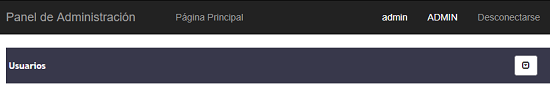
\includegraphics[
   keepaspectratio=true
]{./11_Apendice/Apendice_B/img/WebPanelUsuarios1.png}
\caption{Pantalla administración usuarios - Panel de administración}
\end{figure}

Haciendo click sobre el botón que aparece a la derecha de la entidad, se mostrarán los correspondientes datos almacenados. Se mostrarán en formato tabla, siendo las columnas los atributos de la entidad.


\begin{figure}[H]
\centering
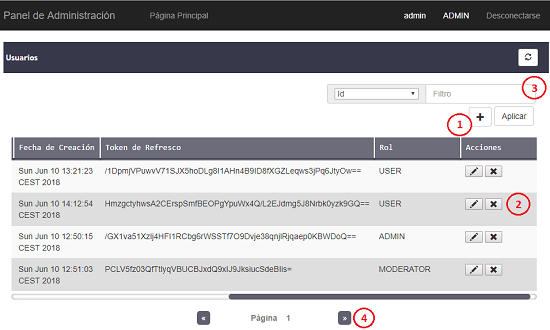
\includegraphics[
   keepaspectratio=true
]{./11_Apendice/Apendice_B/img/WebPanelUsuarios2.png}
\caption{Pantalla administración usuarios - Panel de administración}
\end{figure}

En la figura se diferencian cuatro zonas.


\begin{itemize}
	
	\item \textbf{Zona 1. }Botón que permite dar de alta un nuevo elemento a la entidad. Muestra la siguiente ventana emergente con el formulario a cubrir.
	
\begin{figure}[H]
\centering
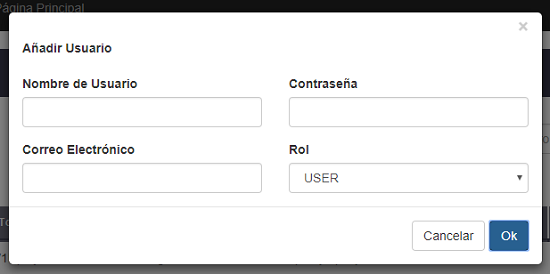
\includegraphics[
   keepaspectratio=true
]{./11_Apendice/Apendice_B/img/WebPanelUsuariosAdd.png}
\caption{Pantalla añadir usuario - Panel de administración}
\end{figure}

El administrador indicará los datos necesarios y confirmará la acción.
	
	\item \textbf{Zona 2. }Muestra el conjunto de acciones a realizar sobre cada elemento de la tabla. Incluye:
	\begin{itemize}
		\item \textbf{Editar. }Botón con el icono de un lápiz. Muestra una ventana con los datos de dicho elemento, permitiendo realizar modificaciones sobre ellos. Los campos ensombrecidos no pueden ser modificados.
		
		\begin{figure}[H]
		\centering
		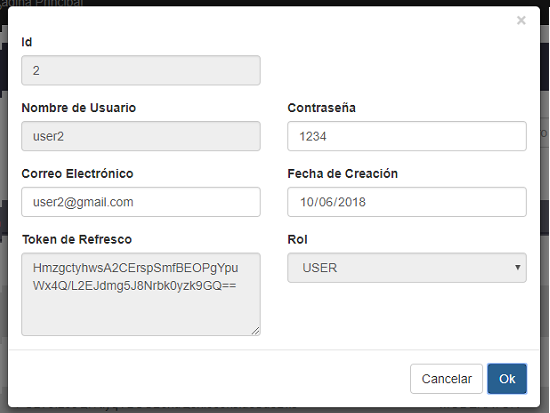
\includegraphics[
   		keepaspectratio=true
		]{./11_Apendice/Apendice_B/img/WebPanelUsuariosEdit.png}
		\caption{Pantalla modificar usuario - Panel de administración}
		\end{figure}
		
		\item \textbf{Eliminar. }Icono con el botón de una aspa. Muestra una ventana pidiendo confirmación para eliminar dicho elemento.
		\begin{figure}[H]
		\centering
		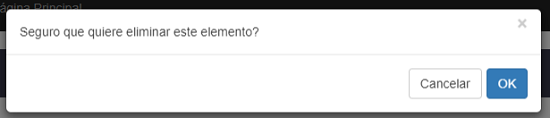
\includegraphics[
   		keepaspectratio=true
		]{./11_Apendice/Apendice_B/img/WebPanelUsuariosDel.png}
		\caption{Pantalla eliminar usuario - Panel de administración}
		\end{figure}
	\end{itemize}		
	
	\item \textbf{Zona 3. }Formada por un selector, un input y un botón de \textit{Aplicar}. En el selector se selecciona el atributo de la entidad sobre el cual se aplicará un filtro, en el input se indicará el valor por el que filtrar y accionando el botón se aplicará dicho filtro sobre la tabla.
	
	\item \textbf{Zona 4. }Indica la paginación de la tabla. Haciendo uso de las flechas, adelante y atrás, se podrán obtener los datos de la entidad de forma paginada.
\end{itemize}


Para el resto de entidades a administrar, las acciones serán las mismas que las representadas en la entidad anterior. Únicamente mencionar, que para las entidades que gestionan datos de Foursquare (Lugares y Categorías), no se incluirán opciones para dar de alta elementos en estas tablas, solamente, se habilitará la opción, en categorías, para obtenerlas de la fuente externa y añadir dichos datos a la aplicación.

\begin{figure}[H]
\centering
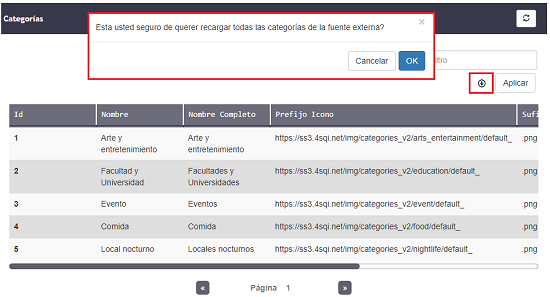
\includegraphics[
keepaspectratio=true
]{./11_Apendice/Apendice_B/img/WebPanelCat.png}
\caption{Pantalla categorías - Panel de administración}
\end{figure}


